% ---------------------------------------------------------------
\subsection{Task 2.3 -- Five-constant model $\qpp=n_1\dTsat^{n_2}(g+n_4\gen\gamma)^{n_3}P^{n_5}$}
\label{sec:t23}

\paragraph{Program.}
\code{P2\_Task2.3.ipynb} is a copy of the Task~2.2 program with modifications (i)--(vii) of the
statement (red data uncommented, $N_D=N_S=77$, error function Eq.~(1.7) in the two loops, mating of
$n_4$ and $n_5$, five-constant print-out and plot, initial guesses (vii)). They are listed in
Section~\ref{sec:codechanges}. I also added the 15 validation points of the Appendix (\code{vdata}).
They are never used by the GA; they only test the fitted relation on data it has not seen.

\paragraph{Run with the initial guesses (vii).}
The initial guesses of the statement already give $\Ferrmean=\TwoThreeFinit$. The GA (MUT $=\pm9\,\%$,
NGEN $=6000$) goes below the target 0.03 at generation \TwoThreeBaseKconv\ and reaches a minimum of
\TwoThreeBaseF\ at generation \TwoThreeBaseKmin\ (Table~\ref{tab:t23const}). The target is met. However,
the deterministic check shows that the error function can go down to \TwoThreeRefF, about $25\,\%$
lower, so a broader range of initial guesses was explored.

\paragraph{Range of initial guesses.}
Five sets of initial guesses were run with two mutation amplitudes and five seeds each
(Table~\ref{tab:t23study}):
(A)~the guesses (vii) of the statement;
(B)~no pressure effect ($n_5=0.01$) and the pure-fluid gravity exponent $n_3=0.25$;
(C)~stronger gravity/Marangoni and pressure effects ($n_3=n_5=0.5$, $n_4=2$);
(D)~a far guess;
(E)~all constants equal to 1.
The best single run of each seed was then refined in two more stages, restarted from its best constants
with MUT $=0.03$ and then $0.01$ (last column of Table~\ref{tab:t23study}).

\begin{table}[H]
\centering\scriptsize
\caption{Task 2.3: effect of the initial guesses (NGEN $=6000$, 5 seeds per line, 3 for MFRAC $=1$).
``frac.\ nkeep$=0$'' = fraction of generations without any survivor. ``refined'' = best and worst
$\Ferrmean$ after the two refinement stages (MUT $=0.03$ then $0.01$) for 3 seeds. Deterministic reference
minimum: $\TwoThreeRefF$.}
\label{tab:t23study}
\fittable{t23_study}
\end{table}

The behaviour is richer than for three constants:
\begin{itemize}
  \item \textbf{Set C converges almost immediately} (target reached in 2--3 generations, $\Ferrmean\approx0.022$),
        and its refinement gives the best fit, within $0.6\,\%$ of the true minimum.
  \item \textbf{Set A} (statement) always meets the target, but it stops at $0.025$--$0.030$, and at
        $0.022$--$0.023$ after refinement. It starts with $n_3\approx n_5\approx0.22$, on the wrong
        side of a long valley in the $(n_3,n_5)$ directions, and the population moves along this valley only
        slowly.
  \item \textbf{Set B shows a limitation of multiplicative mutations.} A constant guessed close to zero
        can hardly move: a $\pm9\,\%$ mutation of $n_5=0.01$ changes it by at most $\pm0.0009$. The
        pressure exponent therefore stays close to 0, the other constants have to compensate, and only
        3/10 runs reach the target. \emph{A constant whose sign or order of magnitude is unknown should not
        be initialised close to zero.}
  \item \textbf{Sets D and E fail}, even after refinement ($\Ferrmean\ge0.033$). With Set E and the skeleton
        settings, the population is even \emph{frozen}: in $90\,\%$ of the generations no organism has an
        error below $0.5\times$ median, so \code{nkeep}$\,=0$. All offspring are then mutations of the same
        organism \code{n[0]}, which is never replaced (the median error stays at 0.95). Larger mutations
        (MUT $=0.2$) or a less selective threshold (MFRAC $=1$) unfreeze the population, but 6000
        generations are not enough to reach the valley. The same mechanism is analysed in detail for
        Part~2 (Section~\ref{sec:part2}, Fig.~\ref{fig:t25nkeep}).
\end{itemize}

\paragraph{Best fit.}
The best-fit constants are given in Table~\ref{tab:t23const} (set \TwoThreeBestSet, seed \TwoThreeBestSeed, refined):
\[
\boxed{\qpp=\TwoThreeNone\,\dTsat^{\,\TwoThreeNtwo}\,\bigl(g+\TwoThreeNfour\,\gen\gamma\bigr)^{\TwoThreeNthree}\,P^{\,\TwoThreeNfive}}
\]
with $\Ferrmean=\TwoThreeF$ ($<0.03$) ($\qpp$ in W/cm$^2$, $T$ in \textdegree C, $g$ in m/s$^2$, $P$ in kPa). Figure~\ref{fig:t23evol} shows the evolution
of the constants and of the error. The deterministic check gives $\Ferrmean=\TwoThreeRefF$, with slightly
different constants ($n_2=\TwoThreeRefNtwo$, $n_3=\TwoThreeRefNthree$, $n_4=\TwoThreeRefNfour$,
$n_5=\TwoThreeRefNfive$). The profiles of Fig.~\ref{fig:t23prof} explain this difference. When one
constant is fixed and the four others are re-optimised, the minimum error increases by only $3\,\%$ (to
about 0.0215) over the ranges $n_2\approx2.8$--$3.2$ ($\pm7\,\%$), $n_3\approx0.41$--$0.54$
($\pm14\,\%$), $n_4\approx1.1$--$1.65$ ($\pm20\,\%$) and $n_5\approx0.28$--$0.65$ ($\pm40\,\%$).
The superheat exponent is therefore well determined by the data, $n_3$ reasonably well, and $n_4$ and
$n_5$ only weakly. Constants with this kind of uncertainty can differ between equally good fits. This is
expected for $n_5$: pressures other than 5.5~kPa appear only in two groups, and the 7.0~kPa group is
also the only one with $\gamma=0$.

\begin{table}[H]
\centering\scriptsize
\caption{Task 2.3: constants of Eq.~(1.5). $^\dagger$average of $\Ferrmean$ over all generations.}
\label{tab:t23const}
\fittable{t23_constants}
\end{table}

\begin{figure}[H]
\centering
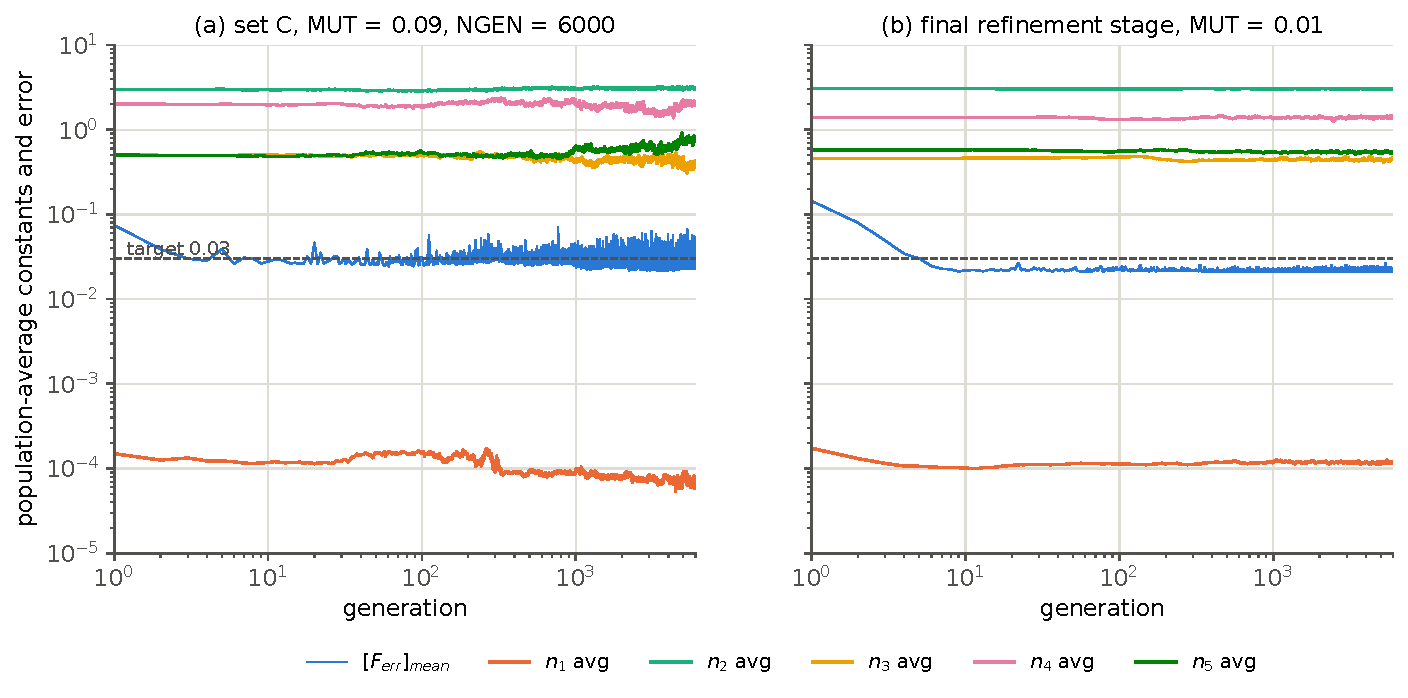
\includegraphics[width=\linewidth]{figures/t23_evolution.pdf}
\caption{Task 2.3: population-average constants and error of the best-fit sequence. (a) Main GA run from
set C; (b) last refinement stage (MUT $=0.01$).}
\label{fig:t23evol}
\end{figure}

\begin{figure}[H]
\centering
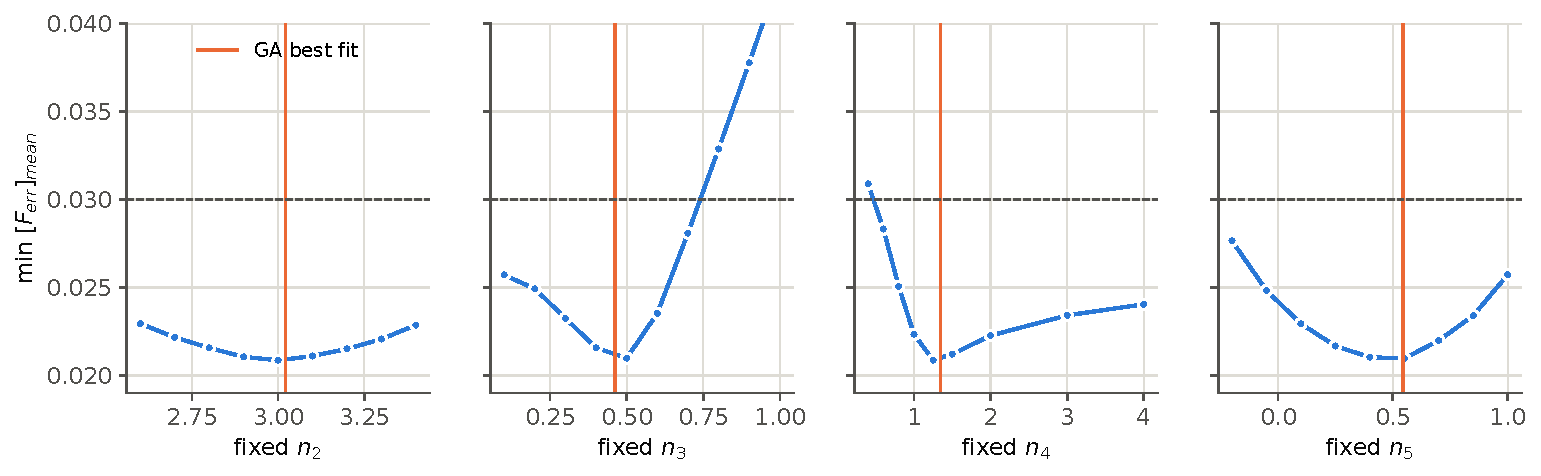
\includegraphics[width=\linewidth]{figures/t23_profiles.pdf}
\caption{Task 2.3: minimum achievable $\Ferrmean$ when one constant is fixed and the four others are
re-optimised. A flat profile means that the data determine this constant only weakly.}
\label{fig:t23prof}
\end{figure}

\paragraph{Quality of the fit and validation.}
Figure~\ref{fig:t23parity} compares the predictions with the 77 training points and the 15
validation points.
\begin{itemize}
  \item Training data: rms fractional deviation $\TwoThreeRmsTrain\,\%$, mean absolute deviation
        $\TwoThreeMadTrain\,\%$, $\TwoThreeWithinTrain\,\%$ of the points within $\pm10\,\%$. For the
        45 points of Task~2.2, the three-constant model gave $16.6\,\%$, $13.2\,\%$ and $47\,\%$.
  \item Validation data: $\Ferrmean=\TwoThreeFval$, rms fractional deviation $\TwoThreeRmsVal\,\%$, mean
        absolute deviation $\TwoThreeMadVal\,\%$.
\end{itemize}
Overall, the deviation is now close to the estimated noise of the data (about $10$--$11\,\%$). The
validation error is only slightly larger than the training error, so the five-constant model does not
over-fit (77 points for 5 constants). The largest validation deviation is the point
$(\qpp,T_w-T_{sat})=(50.9,\ 37.2)$ at $0.01\,\gen$: its superheat is 3\,\textdegree C higher than that of the
training point with almost the same heat flux ($49.4$~W/cm$^2$ at $34.2$\,\textdegree C), which points to measurement scatter.

\textbf{The remaining deviation is not entirely random, however.} Table~\ref{tab:t23bias} gives the mean
deviation of each test condition. Four conditions are fitted within the noise (mean deviation between
$\TwoThreeBiasOthersMin\,\%$ and $\TwoThreeBiasOthersMax\,\%$). Two are still biased: the $1\,\gen$ group
is overpredicted by about $16\,\%$ (mean deviation $\TwoThreeBiasOneG\,\%$) and the $2\,\gen$ group at 5.5~kPa is
underpredicted by about $11\,\%$ (mean deviation $\TwoThreeBiasTwoG\,\%$). The equivalent-gravity term reduces the
gravity bias of Eq.~(1.1) ($-19\,\%$ and $+16\,\%$ for the same two groups) but does not remove it.
With a single exponent $n_3$, the form $(g+n_4\gen\gamma)^{n_3}$ cannot give at the same time almost no
change between $0.01$ and $1\,\gen$ and a $40$--$50\,\%$ increase between $1$ and $2\,\gen$ at 5.5~kPa
(Fig.~\ref{fig:t23parity}). Part of the gravity effect is therefore still missing from Eq.~(1.5), and
predictions at $1$ and $2\,\gen$ carry this systematic error on top of the scatter.

\begin{table}[H]
\centering\small
\caption{Task 2.3: mean and rms deviation $(\qpp_{exp}-\qpp_{pred})/\qpp_{pred}$ for each test condition
(training data). Mean deviations larger than $10\,\%$ are in bold. Last column: the three-constant fit
of Task~2.2 for the groups it was fitted on.}
\label{tab:t23bias}
\fittable{t23_bias}
\end{table}

\begin{figure}[H]
\centering
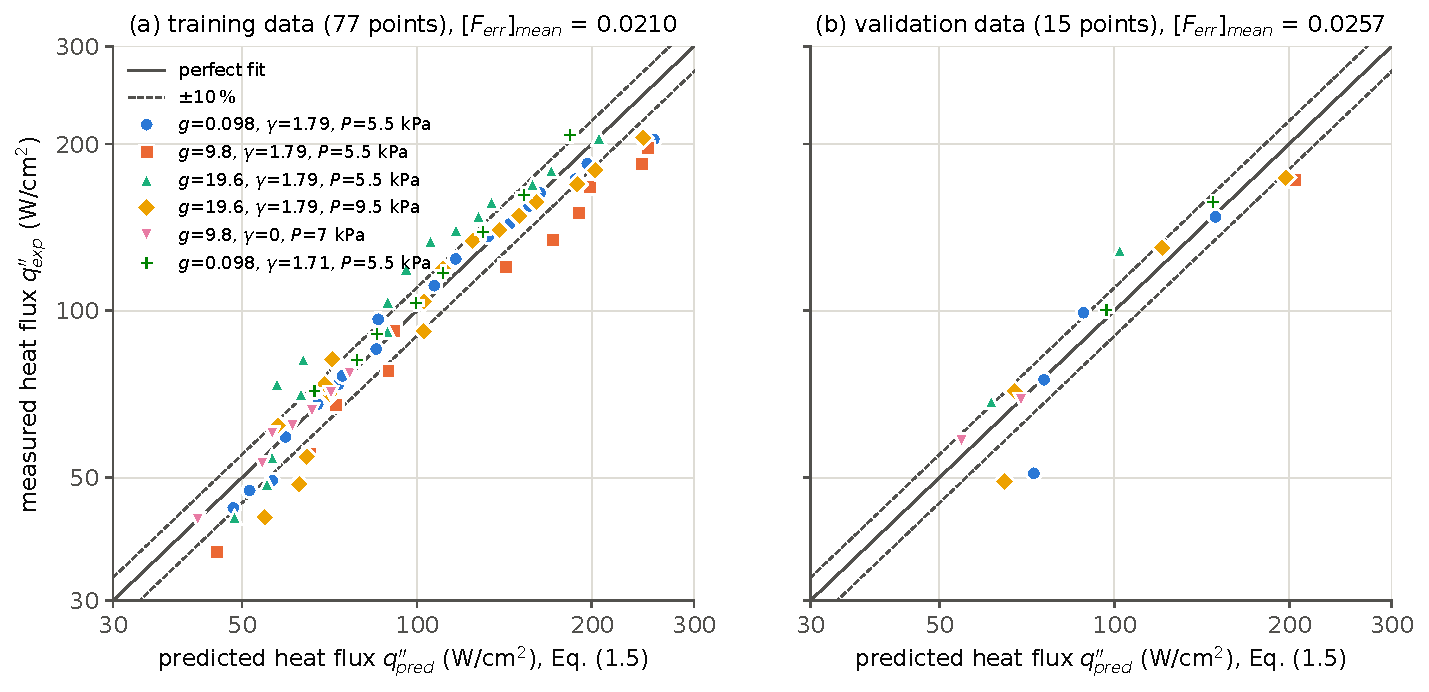
\includegraphics[width=\linewidth]{figures/t23_parity.pdf}
\caption{Task 2.3: measured versus predicted heat flux, Eq.~(1.5) with the best-fit constants. (a) 77
training points; (b) 15 validation points. One symbol per test condition.}
\label{fig:t23parity}
\end{figure}

\paragraph{Surface plot and physical interpretation.}
Figure~\ref{fig:t23surf} shows $\qpp/\dTsat^{n_2}=n_1(g+n_4\gen\gamma)^{n_3}P^{n_5}$ for
$1<g<20$~m/s$^2$ and $0<\gamma<2$ at $P=10$~kPa. Three conclusions follow:
\begin{itemize}
  \item \textbf{The Marangoni effect acts like an additional gravity.} The term $n_4\gen\gamma$ is an
        ``equivalent gravity'' produced by the surface tension gradients. For $\gamma=1.79$ it equals
        $\TwoThreeGeq$~m/s$^2$ ($\approx\TwoThreeGeqRatio\,\gen$), which is larger than earth gravity. This is
        why $\qpp$ depends so little on gravity at low $g$: between $0.01\,\gen$ and $1\,\gen$ the effective
        gravity only goes from about 24 to 33~m/s$^2$. The model still predicts $+17\,\%$ over this range,
        where the data show almost no change (Task~2.1(b)); this is the residual bias of Table~\ref{tab:t23bias}.
  \item \textbf{The gravity dependence depends on $\gamma$.} Without Marangoni effect ($\gamma=0$),
        $\qpp/\dTsat^{n_2}$ increases by a factor of 4 between $g=1$ and $20$~m/s$^2$. For $\gamma=2$ it
        increases by only $27\,\%$. At $g=1$~m/s$^2$, going from $\gamma=0$ to $\gamma=2$ multiplies the
        heat flux by 4.6. This is why a mixture with a positive $\gamma$ is attractive for low-gravity
        applications.
  \item The superheat exponent $n_2\approx3.0$ agrees with Tasks~2.1(b) and 2.2. The positive pressure
        exponent ($n_5\approx0.5$) agrees with the known increase of nucleate boiling heat transfer with
        pressure (through the fluid properties).
\end{itemize}

\begin{figure}[H]
\centering
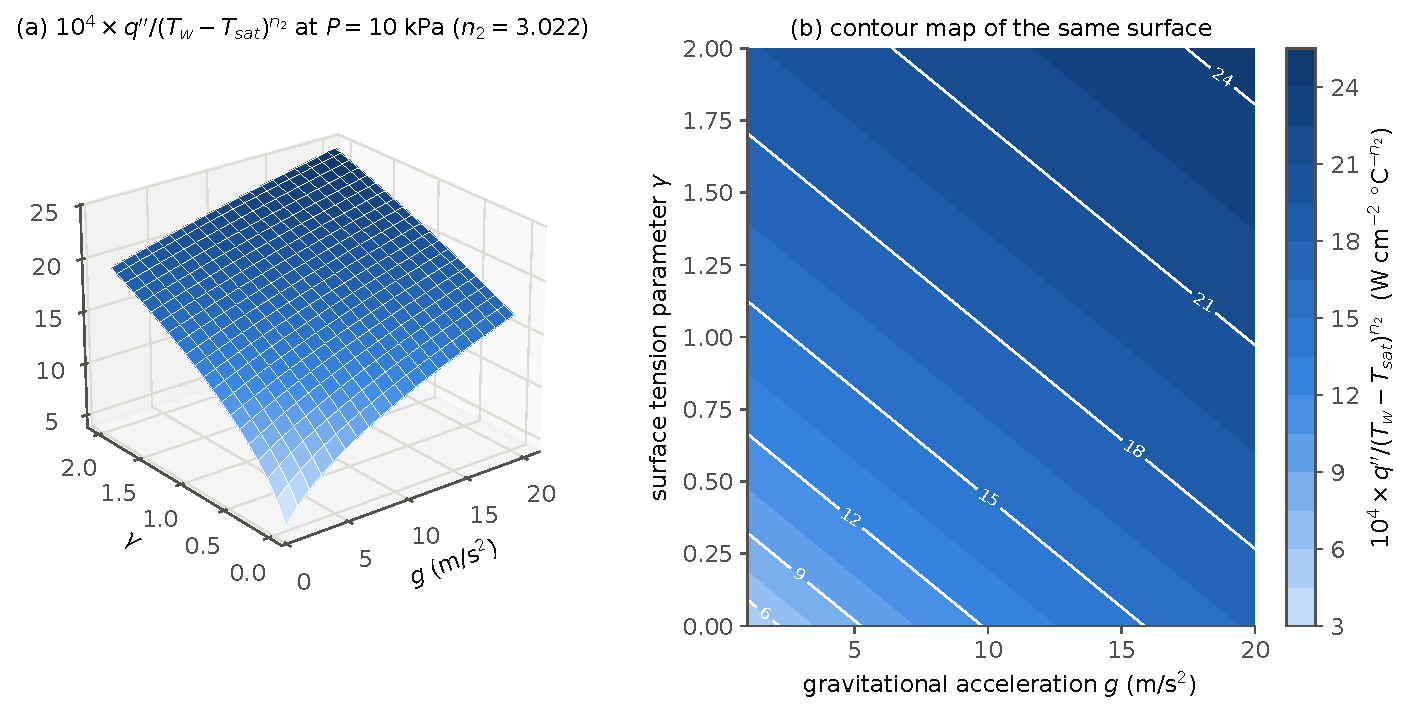
\includegraphics[width=\linewidth]{figures/t23_surface.pdf}
\caption{Task 2.3: $\qpp/\dTsat^{n_2}$ versus $g$ and $\gamma$ at $P=10$~kPa for the best-fit constants:
(a) surface plot; (b) contour map of the same surface.}
\label{fig:t23surf}
\end{figure}
